\section{Processi e procedure al loro supporto}
\subsection{Gestione del progetto}
Come è evidenziato nel capitolo: \hyperref[referenzaRDP]{ruoli}, il \textit{responsabile di progetto} si occuperà di gestire il progetto fino alla sua conclusione. Qui di seguito sono quindi riportate le linee guida quali dovrà attenersi al fine di svolgere un lavoro maggiormente disciplinato ed automatizzato.

\subsubsection{Pianificazione attività}

Il \textit{responsabile di progetto} per ogni attività indicata nel documento \textit{Piano di Progetto} dovrà creare un nuovo progetto seguendo la procedura qui descritta:

\begin{enumerate}
\item Inserire una milestone\ped{G};
\item Inserire le attività da svolgere;
\item Inserire le rispettive sotto-attività;
\item Calcolare ed inserire i periodi di slack\ped{G} qualora fosse necessario;
\item Creare le risorse;
\item Assegnare le risorse create ad ogni attività;
\item Salvare la baseline\ped{G}.
\end{enumerate}

Sarà decisa a discrezione del \textit{Responsabile di Progetto} per ogni attività la possibilità di assegnare un surplus di ore, queste ore supplementari verranno scelte basandosi sulla criticità dell'attività considerata. 
	
\subsubsection{Utilizzo del ticketing}
Ogni membro del team \textit{Sirius} avrà accesso al sistema di \textit{ticketing}. Le figure che invece potranno assegnare ticket sono le seguenti:

\begin{itemize}
\item Il \textit{Responsabile di Progetto} assegnerà i \textit{ticket} di massima importanza cioè quelli correlati allo sviluppo delle attività necessarie all' avanzamento del progetto;
\item Il \textit{Verificatore} potrà assegnare \textit{ticket} allo scopo di segnalare errori di grave entità rilevati durante l'attività di verifica.
\end{itemize}

Di conseguenza i \textit{ticket} sono suddivisi in due macro-categorie:
\begin{itemize}
\item \textit{Ticket} di pianificazione, i quali rappresentano le attività che devono essere svolte per procedere con l'avanzamento del progetto, sono suddivisi in 4 sotto-categorie:
\begin{itemize}
\item \emph{Documento}: che rappresenta una \textit{task} inerente alla redazione di un documento; 
\item \emph{Codice}: che rappresenta una \textit{task} inerente alla stesura di codice;
\item \emph{Verifica}: che rappresenta una \textit{task} inerente all'attività di verifica di un'attività;
\item \emph{Generali}: che rappresenta \textit{tasks} i cui scopi sono svariati ed in genere non ad alta priorità, come ad esempio la ricerca di un determinato \textit{software}.
\end{itemize}
lo svolgimento dell'insieme di tutti i ticket di una \textit{task-list} non porterà alla conclusione della \textit{task-list} stessa, questo poiché è prevista la possibilità di aggiungere durante l'avanzamento del progetto ulteriori \textit{task}, fino a quando il \textit{responsabile di progetto} non ne dichiarerà la conclusione;
\item Ticket di verifica, contenenti gli errori identificati dai \textit{verificatori} a seguito dell'analisi del lavoro svolto da qualche membro del \textit{team}.
\end{itemize}

Ogni membro del \textit{team} sarà tenuto ad utilizzare la barra di avanzamento di stato del \textit{ticket} fornita dall'interfaccia di \textit{TeamWorkPM}, evitando così superflue norme aggiuntive atte a determinare lo stato del \textit{ticket}.

\subsubsection{Creazione di una milestone}
Il \textit{Responsabile di Progetto} dovrà creare una \textit{milestone}, essa indica la data della revisione a cui il gruppo \gruppo{} intende presentarsi, è possibile visualizzare lo stato di avanzamento che tiene conto del numero di \textit{ticket} completati rispetto al numero di \textit{ticket} complessivi.
Per la creazione di una nuova \textit{milestone} il \textit{Responsabile di Progetto} dovrà seguire i seguenti passi:
\begin{enumerate}
\item Aprire il progetto dall'interfaccia \textit{web} di \textit{TeamWorkPM};
\item Posizionarsi sull'opzione: "\emph{Milestones}" ed accedervi;
\item Cliccare sull'opzione: "\emph{Add a new milestone}".
\end{enumerate}

Completati questi passaggi apparirà il seguente \textit{form\ped{G}} (fig 1) che dovrà essere compilato per concludere la creazione della una \textit{milestone}.
\begin{figure}
\centering
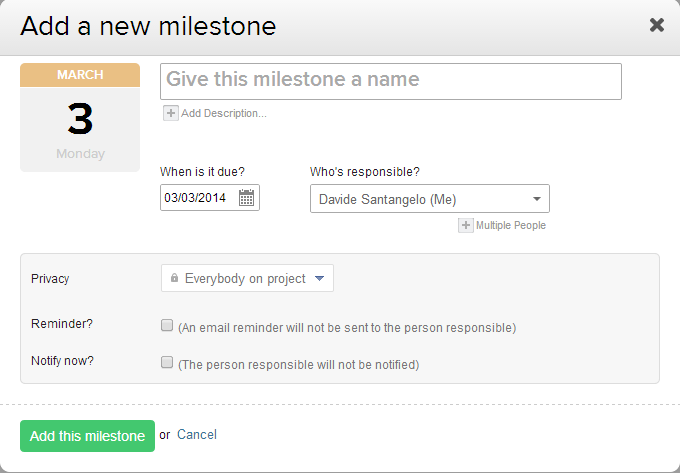
\includegraphics[width=%
\textwidth]{immaginiNDP/Immagine}
\caption[]{Creazione di una milestone.}
\label{fig:Immagine}
\end{figure}

\subsubsection{Procedura di creazione ticket} 
Il \textit{Responsabile di Progetto} dovrà attenersi alla seguente procedura per la creazione di una nuova task-list, ovvero la concretizzazione di un macro-attività e delle sue relative task (ticket). Si ricorda che TeamWorkPM prevede la possibilità di indicare interdipendenze tra task-list.
\begin{enumerate}
\item Dall'interfaccia \textit{web} accedere al progetto \progetto{}, e selezionare dal \textit{menù} principale il comando: \emph{"Task"};
\item Procedere, se necessario, con la creazione di una nuova \textit{task-list} tramite il comando: \emph{"Add task list"};
\item Una volta creata la \textit{task-list} sarà possibile creare i \textit{ticket} (\textit{Task} nel contesto di \textit{TeamWorkPM}) inerenti alla \textit{task-list} scelta.
\end{enumerate}

La struttura di un \textit{ticket} è visualizzabile nella figura 2 di questa sezione.
\begin{figure}
\centering
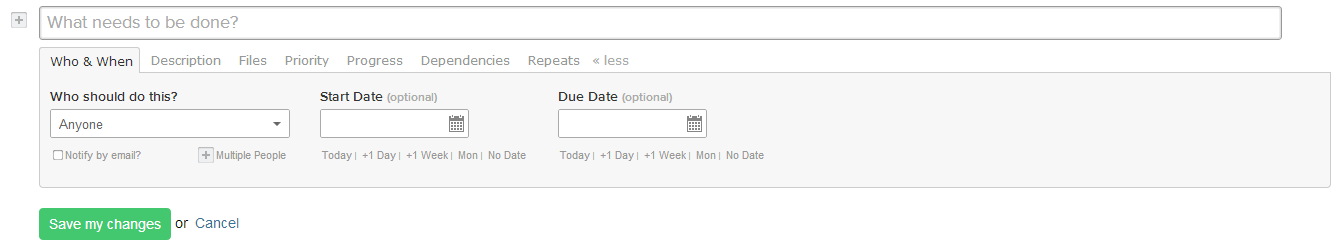
\includegraphics[width=%
\linewidth]{immaginiNDP/creazionetask}
\caption[]{Creazione di un ticket.}
\label{fig:creazionetask}
\end{figure}

Nella task è necessario specificare \textbf{obbligatoriamente}:
\begin{itemize}
\item Il \textbf{Titolo} del \textit{ticket}, dovrà contenere tra parentesi quadre la categoria (per i \textit{ticket} di pianificazione anche la sotto-categoria) di \textit{ticket} di cui si tratta;
\item Il \textbf{Destinatario} del \textit{ticket}, cioè colui a cui è stato assegnato;
\item Le \textbf{Date} di inizio e scadenza del \textit{ticket};
\item Le \textbf{Dipendenze} del \textit{ticket}, che specificano l' eventuale necessità di attendere la terminazione di un insieme di \textit{task} prima di poter svolgere quel determinato compito;
\item Una \textbf{Descrizione} la quale dovrà essere breve e coincisa, ma spiegare efficacemente il lavoro assegnato;
\item La \textbf{Priorità} del \textit{ticket} suddivisa in tre categorie: bassa, media, alta.
\end{itemize}

Compilati i seguenti campi, il \textit{ticket} sarà creato ed inviato regolamentarmene.

\subsubsection{Procedura di terminazione ticket}
Se un \textit{ticket} sarà completato è necessario applicare questa procedura di accertamento:
\begin{enumerate}
\item Il membro del \textit{team} a cui è stato assegnato il \textit{ticket} dovrà spuntare la casella di terminazione su \textit{TeamWorkPM};
\item Durante il controllo giornaliero il \textit{Responsabile di Progetto} controllerà quanto necessario a determinare che il lavoro sia stato effettivamente svolto;
\item Se il lavoro è stato effettivamente svolto, sarà avviato un \textit{ticket} di \emph{Pianificazione} a scopo di verificare il lavoro;
\item Nel caso di irregolare svolgimento del \textit{ticket} o problemi di grave entità, il \textit{Responsabile di Progetto} dovrà applicare la procedura di modifica o riassegnazione del \textit{ticket} presente nel prossimo paragrafo;
\item Nel caso di esito positivo (cioè con regolare svolgimento) il \textit{ticket} sarà concluso ed archiviato, mentre al contempo, qualora fosse necessario, saranno avviati dei \textit{ticket} di \emph{Verifica} per la correzione degli errori non gravi rilevati durante la \textit{Verifica};

\end{enumerate}

\subsubsection{Procedura per la modifica o riassegnazione ticket} 
Durante il suo ciclo di vita un \textit{ticket} per varie ragioni può andare in contro a modifiche, è necessario quindi normare la seguente procedura:
\begin{enumerate}
\item Aprire il progetto dall'interfaccia \textit{web} di \textit{TeamWorkPM};
\item Selezionare il \textit{ticket} di interesse;
\item Selezionare il comando: \emph{"Edit Task"};
\item Aggiungere una descrizione riguardo la modifica effettuata;
\item Avvertire l'interessato che è stata effettuata una modifica inserendo: "(MOD)" sul titolo del \textit{ticket}, e qualora fosse necessario reimpostandone la sua priorità.
\end{enumerate}

\subsection{Analisi dei requisiti}
Il documento di \textit{Analisi dei requisiti} sarà sviluppato dagli \textit{Analisti} i quali dovranno attenersi alle regole riportate in questa sezione.

\subsubsection{Classificazione dei requisiti}
Ogni requisito deve essere definito tramite  una descrizione testuale e un codice identificativo, classificante e univoco avente la seguente forma:

\begin{center}\{Tipologia\}\{Importanza\}\{Categoria\}\{Identificatore\}\end{center}


\begin{itemize}

\item Tipologia:
\begin{itemize}
\item \textbf{F:} requisito funzionale;
\item \textbf{Q:} requisito di qualità;
\item \textbf{V:} requisito di vincolo;
\end{itemize}

\item Importanza:
\begin{itemize}
\item \textbf{OB:} requisito obbligatorio;
\item \textbf{DE:} requisito desiderabile;
\item \textbf{OP:} requisito opzionale;
\end{itemize}


\item Categoria:
\begin{itemize}
\item \textbf{U:} requisito funzionale riguardante la parte utente;
\item \textbf{L:} requisito funzionale riguardante la parte utente autenticato;
\item \textbf{A:} requisito funzionale riguardante la parte process owner;
\item vuoto se il requisito è di qualità oppure di vincolo;
\end{itemize}


\item Identificatore è un codice gerarchico composto da uno o più numeri separati da un punto, in cui l'ultimo numero è un identificatore incrementale intero.\\
La rimanente parte di codice viene utilizzata quando il requisito da definire è sotto-requisito di un altro, e identifica il requisito gerarchicamente superiore.

\end{itemize}

\subsubsection{Casi d'uso}
Per ciascun caso d'uso deve essere fornito un codice identificativo, una descrizione testuale e un diagramma UML.

\begin{flushleft}
Il codice identificativo deve rispettare la seguente forma:
\end{flushleft}

\begin{center}UC\{Tipologia\}\{Identificatore\}\end{center}
Tipologia può essere U, L o A, che stanno rispettivamente per utente non autenticato, utente autenticato e process owner.\\
Identificatore è un codice gerarchico composto da uno o più numeri separati da un punto, in cui l'ultimo numero è un identificatore incrementale intero.
La rimanente parte di codice viene utilizzata quando il caso d'uso da definire è una specifica o estensione di un altro, e identifica il caso d'uso gerarchicamente superiore.

\begin{flushleft}
La descrizione deve contenere i seguenti dettagli:
\end{flushleft}

\begin{itemize}
\item Descrizione del caso d'uso;
\item Attori coinvolti;
\item Precondizione;
\item Scenario principale dello svolgersi degli eventi;
\item Senari alternativi;
\item Post-condizione.
\end{itemize}

\begin{flushleft}
Il diagramma deve rispettare le regole della notazione UML 2.x\ped{G}.
\end{flushleft}

\subsection{Progettazione}
Questa sezione descrive le norme cui i progettisti dovranno attenersi durante la stesura del documento:  \textit{Specifica tecnica} ed il documento \textbf{definizione di prodotto}. Queste norme sono dettate al fine di poter redigere un documento il più possibile formale e senza ambiguità.

\subsubsection{Specifica tecnica}
\paragraph{Diagrammi}
Per quanto concerne i diagrammi sarà adottato il linguaggio \textit{Unified Modelling Language}(UML) 2.0,
tramite questo linguaggio si andranno a definire:
\begin{itemize}
\item \textbf{Diagrammi dei package}: ossia elementi di raggruppamento di classi. Tali elementi dovranno figurare durante la progettazione generale e dovranno essere identificati univocamente al fine di stabilire come i suddetti interagiscono tra di loro.

\item \textbf{Diagrammi di sequenza}: I quali andranno a descrivere come un gruppo di oggetti andranno a collaborare per implementare collettivamente un comportamento;

\item \textbf{Diagrammi di attività}: Atti a mostrare i flussi di attivit che gli utenti potranno percorrere durante l'uso dell'applicazione;

\item \textbf{Diagrammi delle classi}: I quali consentono di descrivere tipi di entità con le loro caratteristiche.
\end{itemize}

\paragraph{Design pattern}
Per ogni design pattern utilizzato sarà necessario andare a definire i seguenti punti:
\begin{itemize}
\item Una \textbf{descrizione generale} che riporta la struttura del design pattern scelto;
\item Una \textbf{motivazione} che descriva i vantaggi che ne comporta il suo uso;
\item Il \textbf{contesto applicativo} che associa ai design pattern utilizzati il contesto dove sono stati adottati.
\end{itemize}

\paragraph{Nomenclatura delle classi}
Ogni classe descritta nel documento specifica tecnica seguirà il seguente schema:
\begin{itemize}
\item \textbf{Nome}: enuncia il nome della classe che andrà descritta, devono essere obbligatoriamente in inglese e devono comparire con l'iniziale in maiuscolo.
\item \textbf{Package}:enuncia il pacchetto, ed i relativi sotto-pacchetti, all'interno dei quali è contenuta la classe di interesse.
Ogni package deve seguire la seguente notazione: Pack1::Pack2::..::Pack-n;
ove con:
\begin{itemize}
\item Pack1, si intende il package principale;
\item Pack(x)::Pack(y) indica che indica che y è sotto package di x;
\end{itemize}

\item \textbf{Descrizione}: deve contenere una breve ma significativa descrizione testuale riguardante l'utilizzo della classe;
\item \textbf{Relazione con altri componenti}: viene specificato se la classe di interesse ha relazioni con le classi di altri componenti.
\end{itemize}

\paragraph{Tracciamento}
Ogni componente sarà tracciato seguendo tali regole:\\
\begin{center}
{\textbf{Ambito}}{\textbf{Utente}}{\textbf{Codice}}
\end{center}

ove \textbf{Ambito} rappresenta con:
\begin{itemize}
\item \textbf{V}: view;
\item \textbf{CP}: client presenter;
\item \textbf{SP}: server presenter;
\item \textbf{CM}: client model;
\item \textbf{SM}: server model.
\end{itemize}

ove \textbf{Ambito} rappresenta:
\begin{itemize}
\item \textbf{A}: process owner;
\item \textbf{U}: utente;
\end{itemize}

Per quanto concerne il codice, si adotteranno i codici del tracciamento degli UC.

\subsubsection{Test} I progettisti avranno il compito di definire delle classi e dei test fittizi con lo scopo di valutare il lavoro svolto.
I test saranno suddivisi in:
\begin{itemize}
\item Test di integrazione;
\item Test di unità;
\end{itemize}

\paragraph{Tracciamento requisiti-componenti}

\begin{itemize}
\item \textit{Requisito}: contiene il codice univoco e classificante del requisito;
\item \textit{Descrizione requisito}: contiene la descrizione del requisito;
\item \textit{Nome componente}: contiene il codice identificativo del componente.
\end{itemize}

\paragraph{Tracciamento componenti-requisiti}
La struttura della tabella sarà la seguente:
\begin{itemize}
\item \textit{Requisito}: contenente il codice univoco e classificante del requisito;
\item \textit{Componente}: contente il nome del package ed il nome della classe.
\end{itemize}

\paragraph{Test di sistema ed integrazione}
Il tracciamento dei test sarà inserito in forma tabellare nel documento \PianoDiQualifica, e dovrà rispettare il seguente stampo:
\begin{itemize}
\item \textbf{Codice test}: il quale dovrà essere obbligatoriamente univoco ed atto ad identificare il test;
\item \textbf{Descrizione}: la quale specifica lo scopo del test;
\item \textbf{Requisito annesso}: che specifica il requisito cui il test fa riferimento;
\item \textbf{Stato}: che riporta se il test è stato effettuato.
\end{itemize}

\subsubsection{Definizione di prodotto}
Redigere il documento di \textit{definizione di prodotto} sarà compito dei \textit{progettisti}.
La \textit{definizione di prodotto} è un documento che si pone l'obbiettivo di definire dettagliatamente ogni singola unità di cui è composto il sistema. Al fine di non lasciare libertà di iniziativa durante l'attività di codifica sarà necessario quindi specificare i metodi e gli  attributi di ogni classe.

\paragraph{UML}\begin{flushleft}
Qusto documento presenterà una versione più raffinata, rispetto alla specifica tecnica, dei seguenti diagrammi:
\end{flushleft}
\begin{itemize}
\item \textbf{Diagrammi delle classi};
\item \textbf{Diagrammi di sequenza}.
\end{itemize}

\paragraph{Formalismo delle classi}\begin{flushleft}
Ogni classe deve essere definita attenendosi alle seguenti convenzioni:
\end{flushleft}
\begin{itemize}
\item \textbf{attributi:} dovranno essere indicati specificando il grado di accessibilità come previsto da UML 2.4. Infine dovrà seguire (riportata sotto il diagramma) la descrizione dell'attributo stesso.
\item \textbf{metodi:} come per gli attributi si dovrà specificare il grado di accessibilità dei suddetti, a seguito dovrà figurare il nome del metodo stesso. Tra parentesi tonde si dovranno inserire i suoi parametri. Infine si inserirà il tipo di ritorno del metodo.
\item \textbf{Parametri:} i parametri, racchiusi da parentesi tonde, devono presentare il loro nome seguito da due punti ed il loro tipo.
\end{itemize}

\subsection{Verifica}
Durante l'intero sviluppo del progetto sarà condotta l'attività di verifica per processi, documenti ed applicazione.
In questo capitolo si disporrano le modalità operative necessarie ai \textit{verificatori} per svolgere l'attività in modo uniforme e disciplinato.

\subsubsection{Tecniche di analisi statica}
L'analisi statica è una tecnica di analisi applicabile sia alla documentazione che al codice e permette di effettuare la verifica di quanto prodotto individuando errori ed anomalie. Essa può essere svolta in due modi diversi ma complementari tra di loro in quanto per utilizzare \textit{inspection} bisogna prima aver effettuato \textit{walkthrough}
\paragraph{Inspection}
Questa tecnica, di analisi statica, consiste nella verifica di sezioni ben definite di un documento o del codice. Questo tipo di controlli per i documenti sono usualmente definiti tramite una lista di controllo (checklist) redatta anticipatamente rispetto all'attività di verifica da intraprendere. Per la verifica dei documenti, la lista di controllo è stata elaborata a seguito di analisi eseguite tramite \textit{walkthrough}, ed evidenziando gli errori più ricorrenti riscontrati. \textit{Inspection} è una strategia rapida in quanto permette l'analisi di alcuni parti ritenute critiche nella checklist senza bisogno di una lettura integrale di documento o di tutto il codice in oggetto.
\paragraph{Walkthrough}
\textit{Walkthrough} è una tecnica di analisi statica che consiste nella lettura critica a largo raggio di tutto il documento. In questa tipologia di analisi il \textit{Verificatore} utilizza molto tempo per la lettura e correzione del documento o codice. Questa tecnica viene di solito utilizzata nella prima parte dello sviluppo di progetti in quanto, la poca esperienza del \textit{Verificatore} non permette un'altro tipo di verifica. Al termine di questo primo set di analisi \textit{walkthrough} viene usualmente definita una lista di controllo che permetta di ricercare in primo luogo gli errori più ricorrenti, e maggiormente riscontrati. \textit{Walkthrough} è un'attività onerosa e collaborativa che richiede l'intervento di più persone per essere efficiente ed efficace

\subsubsection{Tecniche di analisi dinamica}
L'analisi dinamica si applica solamente al prodotto software e consiste nell'esecuzione del codice mediante l'uso di test predisposti per verificarne il funzionamento o rilevare possibili difetti di implementazione eseguendo tutto o solo una parte del codice.
La \textbf{ripetibilità} del test è una caratteristica fondamentale per questo tipo di test, in quanto dichiara che il codice con un certo \textit{input} produce sempre lo stesso \textit{output} su uno specifico ambiente. In questo modo si è in grado di riscontrare problemi e verificare la correttezza del prodotto.
Per questo \gruppo ~ha deciso di definire a priori le seguenti caratteristiche:
\begin{itemize}
\item \textbf{Ambiente}: sistema \textit{hardware} e quello \textit{software} sui quali è stato pianificato l'utilizzo del prodotto, di essi si deve definire uno stato iniziale dal quale poter iniziare ad eseguire i test;
\item \textbf{Specifica di \textit{input}}: definire quali sono gli \textit{input} e quali devono essere gli \textit{output} attesi;
\item \textbf{Procedure}: definire quali devono essere i test ed in che ordine devono essere analizzati i risultati ottenuti.
\end{itemize}
Di seguito sono definiti cinque diversi tipi di test.
\paragraph{Test di unità} 
Per test di unità si intende la verifica di ogni singola unità di prodotto software tramite l'utilizzo di stub\ped{G}, driver\ped{G} e logger\ped{G}. Per unità si intende la più piccola porzione di codice che è utile verificare singolarmente e che viene prodotta da un unico programmatore. Tramite questo tipo di test si vogliono testare i vari le unità per rilevare errori di implementazione da parte dei programmatori.

\paragraph{Test di integrazione}
I test di integrazione prevedono la verifica dei componenti del sistema che vengono aggiunti incrementando il prodotto di origine e si prefigge quindi di analizzare la combinazione di due o più unità software che hanno quindi superato i test di unità. Questa tecnica di verifica serve ad individuare errori residui nella programmazione dei singoli moduli: come modifiche delle interfacce e comportamenti inaspettati di componenti software di parti terze e che pregiudicherebbero la validità del prodotto. Per effettuare tali test può essere necessario l'aggiunta di componenti software fittizie e non ancora implementate al fine di non pregiudicare negativamente l'esito dell'analisi.
\paragraph{Test di sistema}
Consiste nella validazione del sistema attraverso la verifica della copertura di tutti i requisiti obbligatori individuati in \infoAR, e tracciati  grazie allo strumento messo a punto da \gruppo;
\paragraph{Test di regressione}
I test di regressione vengono eseguiti quando si apportano delle modifiche a parte del software e questi consistono nella riesecuzione dei test riguardanti le i componenti che hanno subito modifiche e che precedentemente non erano soggetti ad errori.
Tale operazione viene aiutata dal tracciamento, che permette di individuare e ripetere facilmente i test di unità, integrazione ed eventualmente di sistema che sono stati potenzialmente influenzati dalle modifiche.
\paragraph{Test di accettazione}
Si tratta del collaudo del prodotto software sotto il controllo del proponente. Se il collaudo viene superato in modo positivo, il sistema viene rilasciato e la commessa si conclude.

\subsubsection{Metriche}
I dati rilevati durante l'attività di verifica devono essere analizzati tramite precise metriche.
Con questo termine si intende l'insieme di parametri misurabili su un processo. Qualora le metriche definite in questo documento siano approssimative e/o ambigue, queste dovranno essere ridefinite in modo specifico e seguiranno in modo incrementale il ciclo di vita del prodotto. Di seguito sono riportate le metriche adottate dal team \textit{Sirius}; gli obbiettivi qualitativi che invece definiscono il grado di accettazione/ottimalità verranno riportati nel \PianoDiQualifica{}.

\subsubsection{Metriche per i processi}
Le metriche dei processi ne stabiliscono la qualità, definita come connubio tra \textit{capability}\ped{G}, \textit{maturity}\ped{G} e i miglioramenti. Queste caratteristiche di qualità si possono individuare in tre classi di misure di processo:
\begin{itemize}
\item \textbf{Tempo}: il tempo richiesto per il completamento di un particolare processo;
\item \textbf{Risorse}: le risorse richieste per un particolare processo, in genere vengono definite risorse-uomo, per le risorse software si fa riferimento a \infoNDP;
\item \textbf{Occorrenze}: il numero di volte che capita un particolare evento, che può essere il numero di difetti scoperti durante l'attività di verifica.
\end{itemize}
Per rilevare questi dati \gruppo ~ha deciso di utilizzare, indici che valutano i tempi e i costi del processo. La scelta di queste metriche è dettata anche dal loro possibile utilizzo durante lo svolgimento del processo, per capire in modo semplice se lo stato del processo è conforme a quanto pianificato, mantenendo quindi il processo in controllo. In \infoPDP ~viene specificato come sono stati pianificati questi indici nello stato di avanzamento.
\paragraph{(SV) Schedule Variance}
Indica se si è in linea, in anticipo o in ritardo rispetto alla pianificazione temporale delle attività citata in \infoPDP.
È un indicatore di efficacia temporale e per questo \gruppo ha deciso di esprimerlo in ore.
Se SV $>$ 0 significa che il gruppo di lavoro sta producendo con maggior velocità rispetto a quanto pianificato, viceversa se negativo.\\

\paragraph{(BV) Budget Variance}
Indica se allo stato attuale si è speso più o meno rispetto a quanto pianificato.
È un indicatore che ha valore contabile e finanziario per questo è espresso in euro.
Se BV $>$ 0 significa che l’attuazione del progetto sta consumando il proprio budget con minor velocità rispetto a quanto pianificato, viceversa se negativo.

\subsubsection{Metriche per i documenti}
Come metrica per la verifica dei documenti \gruppo ha deciso di utilizzare l’indice di leggibilità.
Vi sono a disposizione molti indici di leggibilità, ma i più importanti sono per la lingua inglese. Si è deciso quindi di adottare un indice di leggibilità per la lingua italiana.
L’indice \textit{Gulpease} è un indice di leggibilità di un testo tarato sulla lingua italiana. Rispetto ad altri indici, esso ha il vantaggio di utilizzare la lunghezza delle parole in lettere anziché in sillabe, semplificandone il calcolo automatico. Permette di misurare la complessità dello stile di scrittura di un documento.
L’indice viene calcolato utilizzando la formula citata nelle \infoNDP~.
I risultati sono compresi tra 0 e 100, dove il valore 100 indica la leggibilità più alta e 0 la leggibilità più bassa. In generale risulta che testi con un indice:
\begin{itemize}
\item Inferiore a 80 sono difficili da leggere per chi ha la licenza elementare;
\item Inferiore a 60 sono difficili da leggere per chi ha la licenza media;
\item Inferiore a 40 sono difficili da leggere per chi ha un diploma superiore.
\end{itemize}

\subsubsection{Metriche per il software}
Al fine di perseguire gli obiettivi qualitativi dichiarati nel \PianoDiQualifica{} è necessario definire delle metriche, queste metriche hanno quindi l'obbiettivo di rendere quantificabile il lavoro svolto. Questa sezione, però, è da intendersi come modificabile nell'arco dello svolgimento del progetto.

\paragraph{Complessità ciclomatica}
Pensata da T.J. McCabe è utilizzata per misurare la complessità per funzioni, moduli, metodi o classi di un programma. Misura direttamente il numero di cammini linearmente indipendenti attraverso il grafo di controllo di flusso.
Alti valori di complessità ciclomatica indicano una ridotta manutenibilità del codice. Al contrario, valori bassi potrebbero determinare una scarsa efficienza dei metodi. Questo parametro è inoltre un indice del carico di lavoro richiesto dal \textit{testing}. Indicativamente un modulo con complessità ciclomatica più bassa richiede meno test di uno con complessità più elevata.\\
Il valore 10 come massimo di complessità ciclomatica fu raccomandato da T.J.McCabe, l'inventore di tale metrica.
\paragraph{Numero livelli di annidamento}
Rappresenta il numero di livelli di annidamento, quindi l'inserimento di una struttura di controllo all'interno di un'altra. Un elevato valore comporta un'alta complessità e un basso livello di astrazione del codice.\\

\paragraph{Attributi per classe}
Un elevato numero di attributi per classe può rappresentare la necessità di suddividere la classe in più classi, possibilmente utilizzando la tecnica dell'incapsulamento, e può inoltre rappresentare un possibile errore di progettazione.\\

\paragraph{Numero di parametri per metodo}
Un elevato numero di parametri potrebbe richiedere di ridurre le funzionalità del metodo o provvedere ad una nuova progettazione dello stesso.\\

\paragraph{Linee di codice per linee di commento}
Indica il rapporto tra linee di codice e linee di commento: questo parametro è fondamentale per valutare la manutenibilità del codice prodotto, nonché del possibile riuso.\\

\paragraph{Accoppiamento}
\begin{itemize}
\item \textbf{Accoppiamento afferente:} indica il numero di classi esterne al package\ped{G} che dipendono da classi interne ad esso. Un alto valore indica che è presente un alto grado di dipendenza del resto del software dal package. Questo non indica necessariamente una progettazione errata o di bassa qualità, ma possono rappresentare una criticità del package, che quindi perderebbe di robustezza. Al contrario un valore troppo basso potrebbe segnalare che il package analizzato fornisce poche funzionalità e quindi potrebbe risultare scarsamente utile.
\textbf{Parametri utilizzati:}
I valori di range di tale indice verranno definiti durante la progettazione di dettaglio.
\item \textbf{Accoppiamento efferente:} indica il numero di classi interne al package che dipendono da classi esterne ad esso. Mantenendo un basso valore di questo indice, è possibile mantenere il package in grado di garantire funzionalità di base indipendentemente dal resto del sistema.
\end{itemize}
\paragraph{Copertura del codice}
Indica la percentuale di istruzione che vengono eseguite durante i test. Maggiore è la percentuale e più probabilità si hanno di rilevare minori errori nei prodotto. Tale valore può essere abbassato tramite l'utilizzo di metodi molto semplici che non richiedono test.\\

\subsection{Codifica}
\subsubsection{Convenzioni di codifica}
Al fine di produrre codice ordinato e leggibile, in modo da semplificare il più possibile l'attività di manutenzione, per quanto concerne la programmazione \textit{Java\ped{G}}, si adotteranno le norme imposte dalla \textit{Java code conventions}, reperibili all'indirizzo:
\begin{center}
\href{http://www.oracle.com/technetwork/java/codeconvtoc-136057.html}{http://www.oracle.com/technetwork/java/codeconvtoc-136057.html}
\end{center}
Variazioni e modifiche a queste convenzioni possono essere richieste all'\textit{Amministratore}, allegandone la motivazione.
Se l'\textit{Amministratore} riterrà opportune le variazioni presentate, sarà tenuto a notificarlo al team seguendo le convenzioni imposte dalle \textit{Norme di Progetto}.

\subsubsection{Nomi}
Sarà adottata la notazione \textit{CamelCase} al fine di identificare facilmente il nome di variabili, classi, metodi, funzioni, interfacce. Più specificatamente bisognerà rispettare le seguenti regole:
\begin{itemize}
\item \textbf{variabili, metodi, funzioni, interfacce}:dovranno avere la prima lettera minuscola;
\item \textbf{classi}: dovranno avere la prima lettera maiuscola.
\end{itemize}
Inoltre sarà obligatorio utitilizzare la lingua \textbf{inglese} per assegnare i suddetti nomi. 
Inoltre è opportuno ma non obbligatorio che i nomi (di variabili, metodi, etc..) siano esplicativi rispetto al ruolo che assumono nel contesto di applicazione.

\subsubsection{Commenti ed intestazioni}

Ogni file contenente codice dovrà essere provvisto di un intestazione che rispetta la seguente forma:
\\
\\
\textcolor{green}{
\textbf{file}: che riporta il nome del file; \\
\textbf{author}: che riporta il nome dell'autore;\\
\textbf{date}: che riporta la data di creazione; \\
\textbf{lastModified}: che riporta la data di ultima modifica;\\
\textbf{brief}: che descrive brevemente lo scopo e contenuto del file.\\
}

Le classi dovranno obbligatoriamente essere provviste di commenti che contengono:
\\
\\
\textcolor{green}{
\textbf{class}: nome della classe;\\
\textbf{brief}: breve descrizione della classe.\\
}


Per quanto concerne i metodi, essi dovranno essere provvisti di commenti che si adeguano alla seguente forma:
\\
\\
\textcolor{green}{
\textbf{brief}: breve descrizione del compito del metodo;\\
\textbf{param}: che comparirà tante volte quanti sono i parametri in input al metodo, e ne riporterà il nome ed il tipo;\\
\textbf{return}: nome e tipo del valore ritornato dalla funzione.\\}

Infine per le interfacce la forma sarà la seguente:
\\
\\
\textcolor{green}{
\textbf{brief}: breve descrizione dello scopo dell'interfaccia.\\}

Qualora fosse impossibile utilizzare la tecnica del \textit{refractoring}\ped{G} per ristrutturare il codice, nel qualcaso si trattasse di codice particolarmente difficile da comprendere, è possibile dedicare un commento aggiuntivo:
\\
\\
\textcolor{green}{spiegazione approfondita: ...\\}\\
al fine di facilitarne la comprensione.

